%%%----------------------------------------------------------
\chapter{Algebraic Lines, Straight Line Fitting}
%%%----------------------------------------------------------

The focus of this assignment was on understanding the concept of algebraic lines. The task was to create our own class representing Algebraic Lines and some basic utility for it (plotting, distance to a point and intersection between two lines). Then we had to use this class in action for fitting a line to a point cloud as well as segmenting the boundary of a polygon into individual straight lines.

\section{Algebraic lines}

\subsection{Line representation}
A Java class was created which represents an Algebraic Line. I can be described with the following equation:
\begin{equation}
\label{equ:algLineEquation}
	a \cdot x + b \cdot y + c = 0
\end{equation}

The line can be created by either providing the needed parameters $a$, $b$, $c$ or by providing two points. If only two points are provided they are used to calculate the parameters $a$, $b$, $c$ using following equations from the from the lecture notes:
\begin{align}
	a& = -y_2 + y_1 \\
	b& = x_2 - x_1 \\
	x& = -ax_1 - by_1 
\end{align}

\subsection{Plotting}
Lines are usually plotted by defining the two endpoint but since Algebraic Lines has no endpoints we have take a different approach. Instead we used the fact that, if the line is normalized, then 
\begin{equation}
\label{equ:lineEquation}
	ax + by + c = d
\end{equation}
where $d$ represents the perpendicular distance of the point ($x$,$y$)to the line. This means we can iterate over all pixels of the image and check if $d$ is 0. If that is the case that point is on the lane and we can add it to a list. If we color all these points on the list in the end we have our painted line. To be able to draw the line with a specific width $w$ we have to check if $d$ is $w/2$ or smaller instead of $0$.

\subsection{Utility methods}
The three following utility methods were also implemented:
\begin{itemize}
	\item \texttt{void normalize()}: The line is normalized on creation by applying the common scale factor to all three parameters ($a$, $b$, $c$):
	\begin{equation}
		scaleFactor = \frac{1}{\sqrt{a^2 + b^2}} \cdot (a,b,c)
	\end{equation}
	\item \texttt{double distance(Point2D p)}: Returns the perpendicular distance between the line and a provided point by inserting the point's coordinates ($x$,$y$) into equation \ref{equ:lineEquation}.
	\item \texttt{Point2D intersect(AlgebraicLine L2)}: Returns the intersection point of two Algebraic Lines. Since the intersection point is on both lines it also needs to satisfy the equations (\ref{equ:algLineEquation}) of both. We can solve this system of equations by using the matrix-vector notation solving for $p_x$ and $p_y$:
	\begin{equation}
		\begin{pmatrix}
		a_{1} & b_1  \\
		a_{2} & b_2 \\
		\end{pmatrix}
		\cdot
		\begin{pmatrix}
			p_x \\
			p_y \\
		\end{pmatrix}
		=
		\begin{pmatrix}
			-c_1 \\
			-c_2 \\
		\end{pmatrix}
	\end{equation}
\end{itemize}

\subsection{Results}
To test all use cases a test plugin was created which takes a, b, c and desired line width as an input to draw a line. It also draws a line from the upper left corner to the bottom right and draws a circle around the intersection point. It also marks the center of the image red and prints the perpendicular distance from there to the first line created. Figure \ref{fig:Result4_1} shows the outcome.

\begin{figure}
	\centering
	\frame{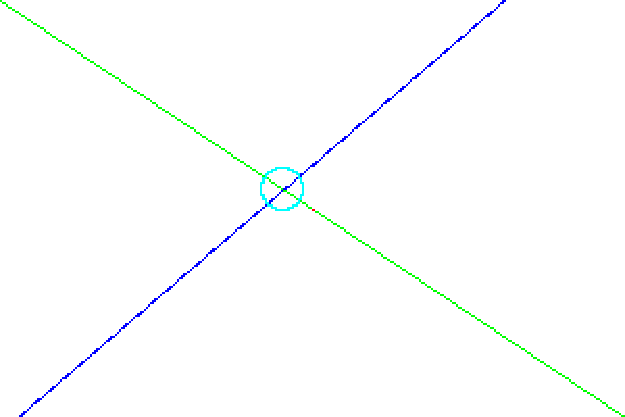
\includegraphics[width=0.6\linewidth]{images/ass04algebraiclines}}
	\caption{The blue line was created with the parameters ($a$, $b$, $c$) The green one with 2 points (upper left corner and bottom right). The intersection point is marked with a cyan circle.}
	\label{fig:Result4_1}
\end{figure}



\section{Fitting a line to a point set}
In this task we had to fit an algebraic line into a given point set using total-least squares minimization. This was achieved by using a method from the lecture notes where the parameters $a$, $b$, $c$ for the best fitting algebraic line are calculated by solving the 2 x 2 eigen-problem. For solving the eigen-problem the class \texttt{imagingbook.lib.math.Eigensolver2x2} was used.
\begin{equation}
	\begin{pmatrix}
		\overline{xx} - \overline{x}^2 & \overline{xy} - \overline{x} \cdot \overline{y} \\
		\overline{xy} - \overline{x} \cdot \overline{y} & \overline{yy} - \overline{y}^2 \\
	\end{pmatrix}
	\cdot
	\begin{pmatrix}
		a \\
		b\\
	\end{pmatrix}
	= \mu
	\begin{pmatrix}
		a \\
		b\\
	\end{pmatrix}
\end{equation}

The resulting vector $(a,b)^T$ is the normal vector to the fitted line. To get $c$ $a$ and $b$ were inserted into the following:
\begin{equation}
	c = -\overline{x} \cdot a - \overline{y} \cdot b
\end{equation}

\subsection{Results}
As we can see in the resulting outcome the algorithm found the best fitting line (\ref{fig:4_2}) and also if we rotate the images for 90 degrees (\ref{fig:4_2_flipped}) the error stays the same.

\begin{figure}
	\centering
	\begin{minipage}[t]{0.32\linewidth}
		\centering
		\frame{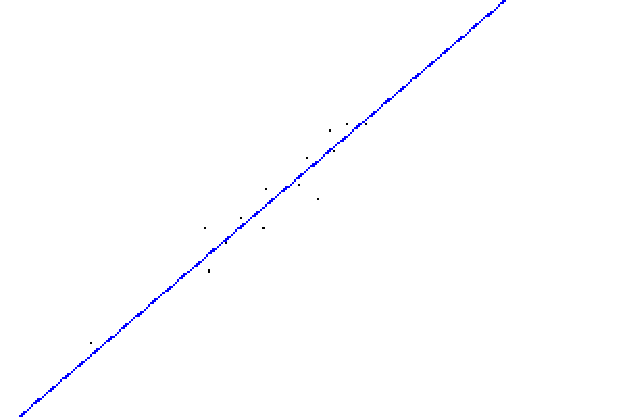
\includegraphics[width=.98\linewidth]{images/ass04line2}}
		\caption{line-test-02 \break a = -0.650719 \break b = -0.759318 \break c = 157.162935 \break error = 618.870335}
		\label{fig:4_2}
	\end{minipage}
	\hfill
	\begin{minipage}[t]{0.32\linewidth}
		\centering
		\frame{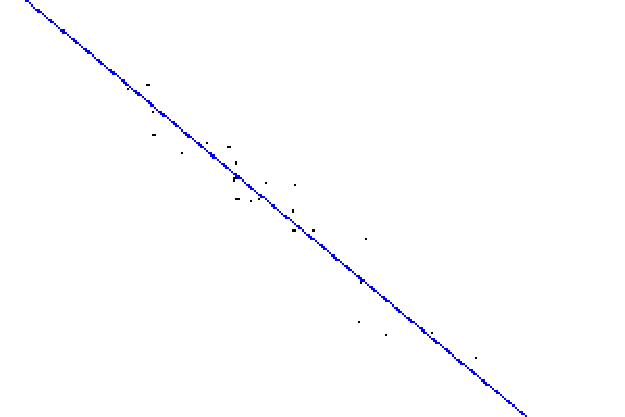
\includegraphics[width=.98\linewidth]{images/ass04line3}}
		\caption{line-test-03 \break a = 0.639506 \break b = -0.768785 \break c = -8.047408 \break error = 1792.254538}
	\end{minipage}
	\hfill
	\begin{minipage}[t]{0.32\linewidth}
		\centering
		\frame{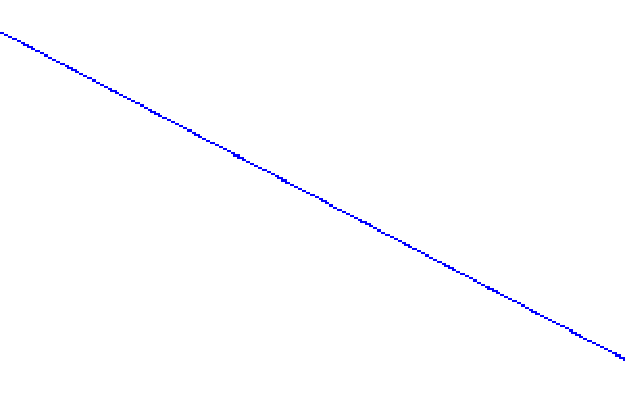
\includegraphics[width=.98\linewidth]{images/ass04line4}}
		\caption{line-test-04 \break a = 0.464632 \break b = -0.885503 \break c = 12.992814\break error = 4.912050}
	\end{minipage}
\end{figure}

\begin{figure}
	\centering
	\begin{minipage}[t]{0.32\linewidth}
		\centering
		\frame{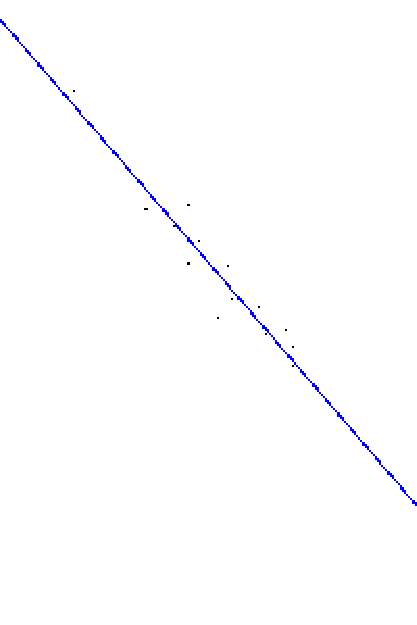
\includegraphics[width=.98\linewidth]{images/ass04line2f}}
		\caption{line-test-02 flipped \break a = -0.759318 \break b = 0.650719 \break c = -37.402258 \break error = 618.870335}
		\label{fig:4_2_flipped}
	\end{minipage}
	\hfill
	\begin{minipage}[t]{0.32\linewidth}
		\centering
		\frame{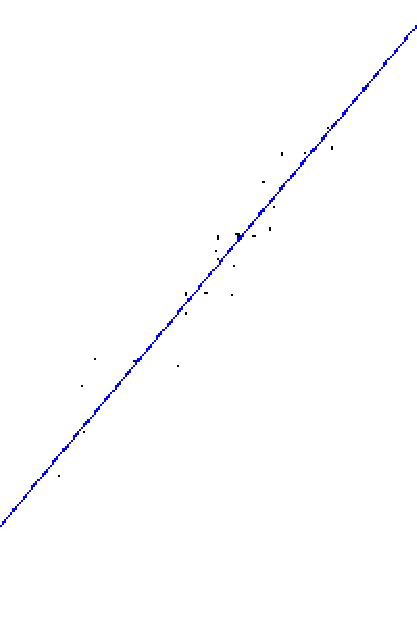
\includegraphics[width=.98\linewidth]{images/ass04line3f}}
		\caption{line-test-03 flipped \break a = -0.768785 \break b = -0.639506 \break c =  183.165052\break error = 1792.254538}
	\end{minipage}
	\hfill
	\begin{minipage}[t]{0.32\linewidth}
		\centering
		\frame{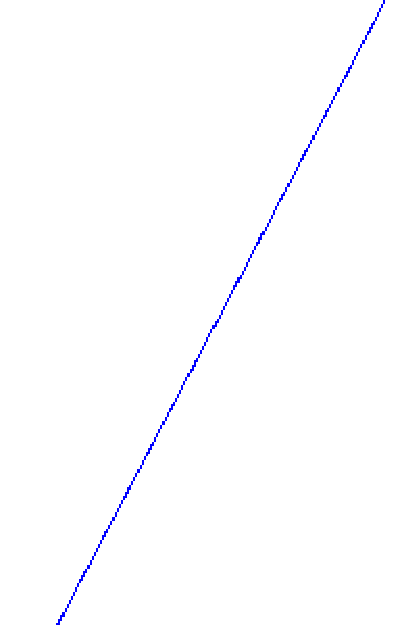
\includegraphics[width=.98\linewidth]{images/ass04line4f}}
		\caption{line-test-04 flipped \break a = -0.885503 \break b = -0.464632 \break c = 151.917798 \break error = 4.912050}
	\end{minipage}
\end{figure}


\section{Segmenting a polygon boundary}
This task was about segmenting the contour pixels of a polygon shape into individual straight line segments. The task was accomplished following these steps:
\begin{enumerate}
	\item Detect the shape and trace its outer contour (assuming that there is only one shape in the image). Collect the contour pixels into a point sequence $P$.
	\item Start at some position in $P$ and start fitting a line after collecting some points.
	\item Keep fitting until the error exceeds a certain limit. As soon as it exceeds remove non-fitting points and start a new line with them.
	\item Continue until all contour pixels are processed.
\end{enumerate}

\subsection{Iterating through contour points}
The contour points are collected using the \texttt{imagingbook.pub.regions} package. At the start of a new line the next 10 points are taken before fitting the line after that the points are  added one by one and the line gets refitted each time.

\subsection{Starting a new line}
As soon as the distance from the current line to the new point is greater than a defined limit a new line is started with the current point as its starting point.

\subsection{Drawing the lines}
The intersection points between the algebraic lines are calculated and then 'normal' lines are drawn between the intersection points.

\subsection{Results}
I had to tinker a bit with the maximum allowed error but after i found the right value it detected the lines pretty well (\ref{fig:Result4_3}). 


\begin{figure}
	\centering
	\frame{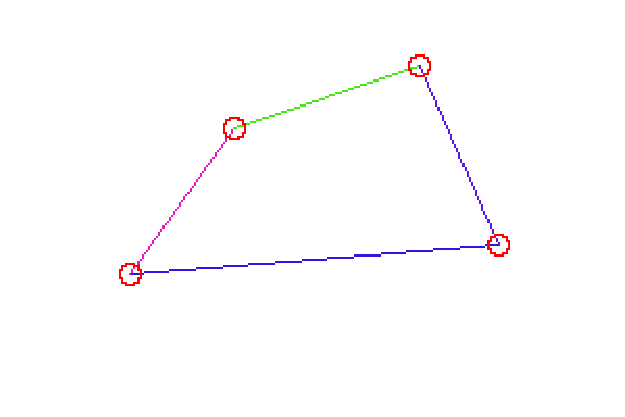
\includegraphics[width=0.6\linewidth]{images/ass04segmentation}}
	\caption{The segmented lines in different colors. The intersection points are marked in red.}
	\label{fig:Result4_3}
\end{figure}






